% !TEX root =  ../report.tex

\section{Scenes}

\begin{figure}
    \caption{Server Selection Page}
    \includegraphics[width=8cm]{content/scenes/Server select.png}  
\end{figure}

\begin{figure}
    \caption{Join Board Overview}
    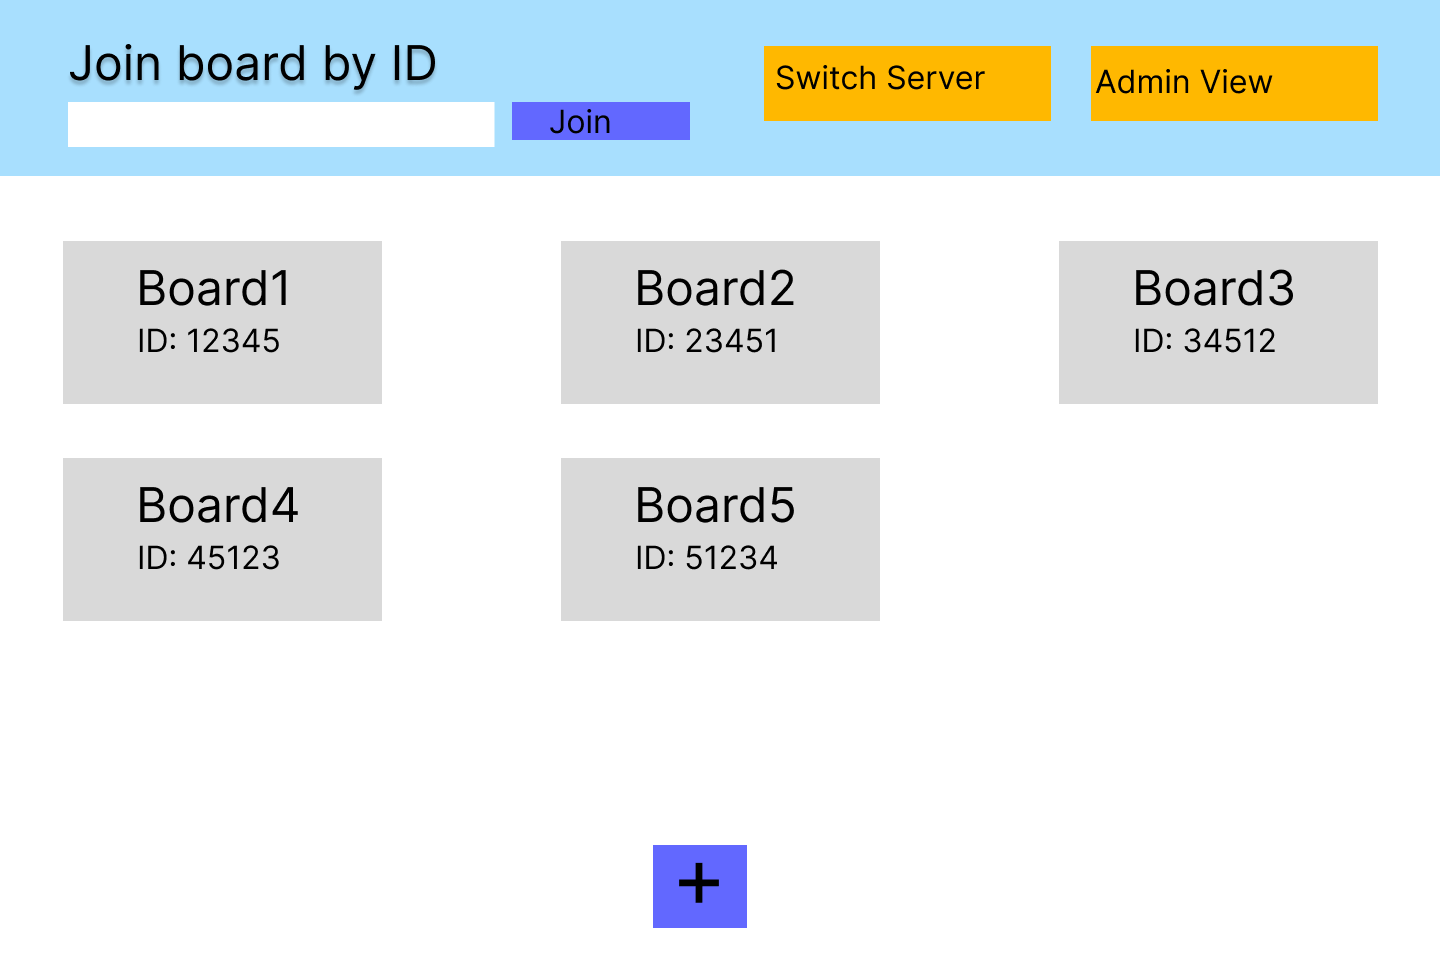
\includegraphics[width=8cm]{content/scenes/Join board overview.png}  
\end{figure}

\begin{figure}
   \caption{Admin Control Panel}
    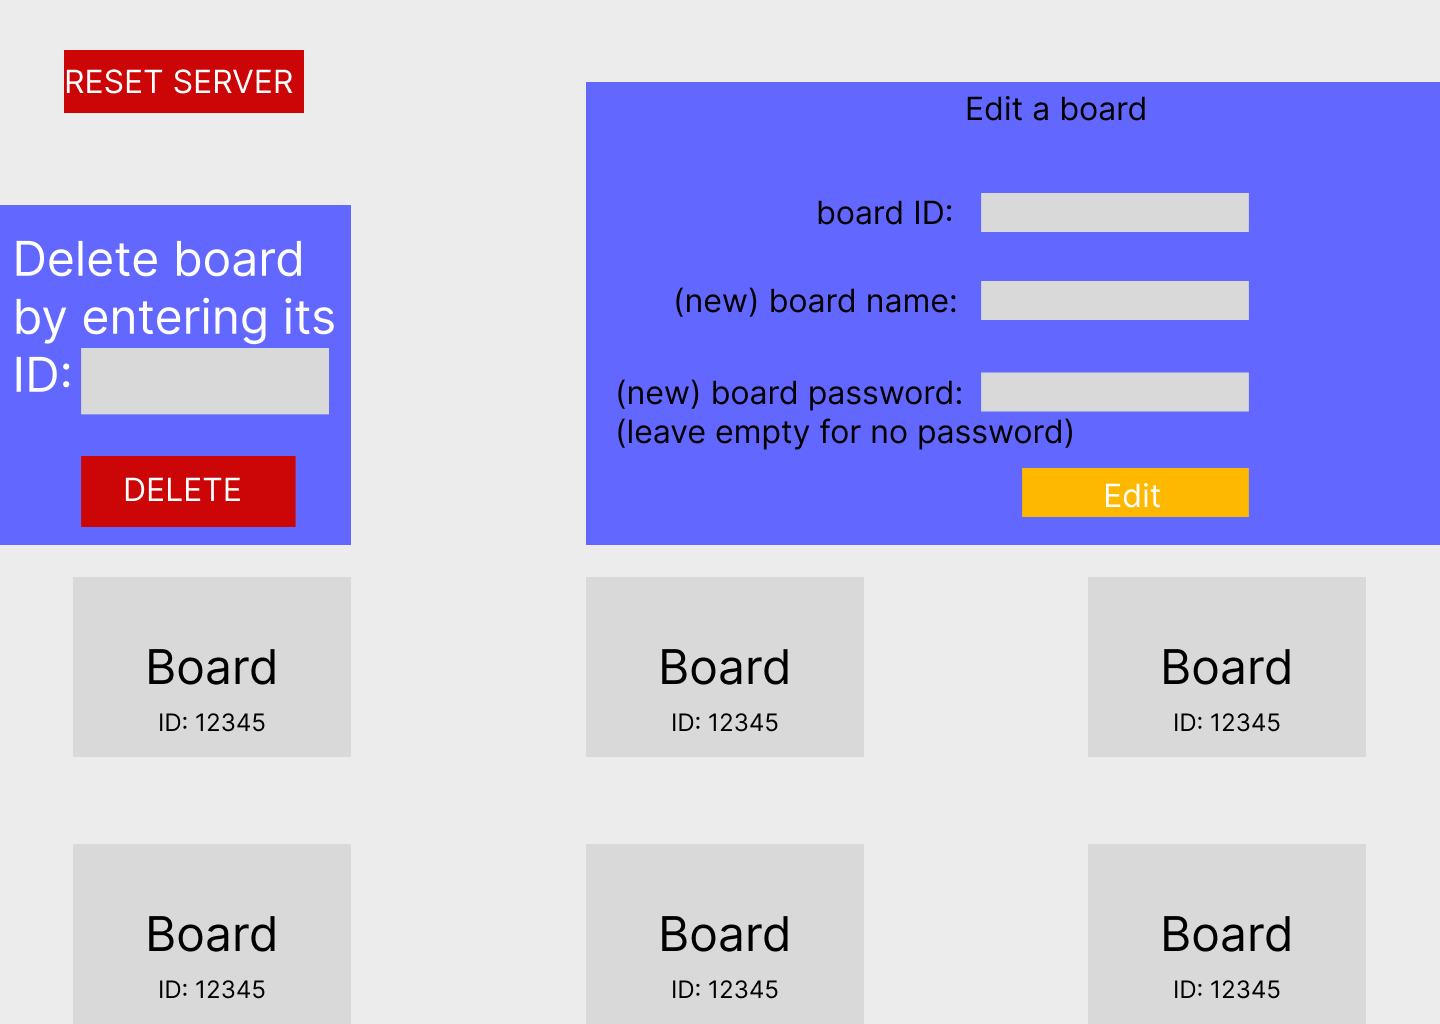
\includegraphics[width=8cm]{content/scenes/Admin Control Panel.png}  
\end{figure}

\begin{figure}
    \caption{Board Overview}
    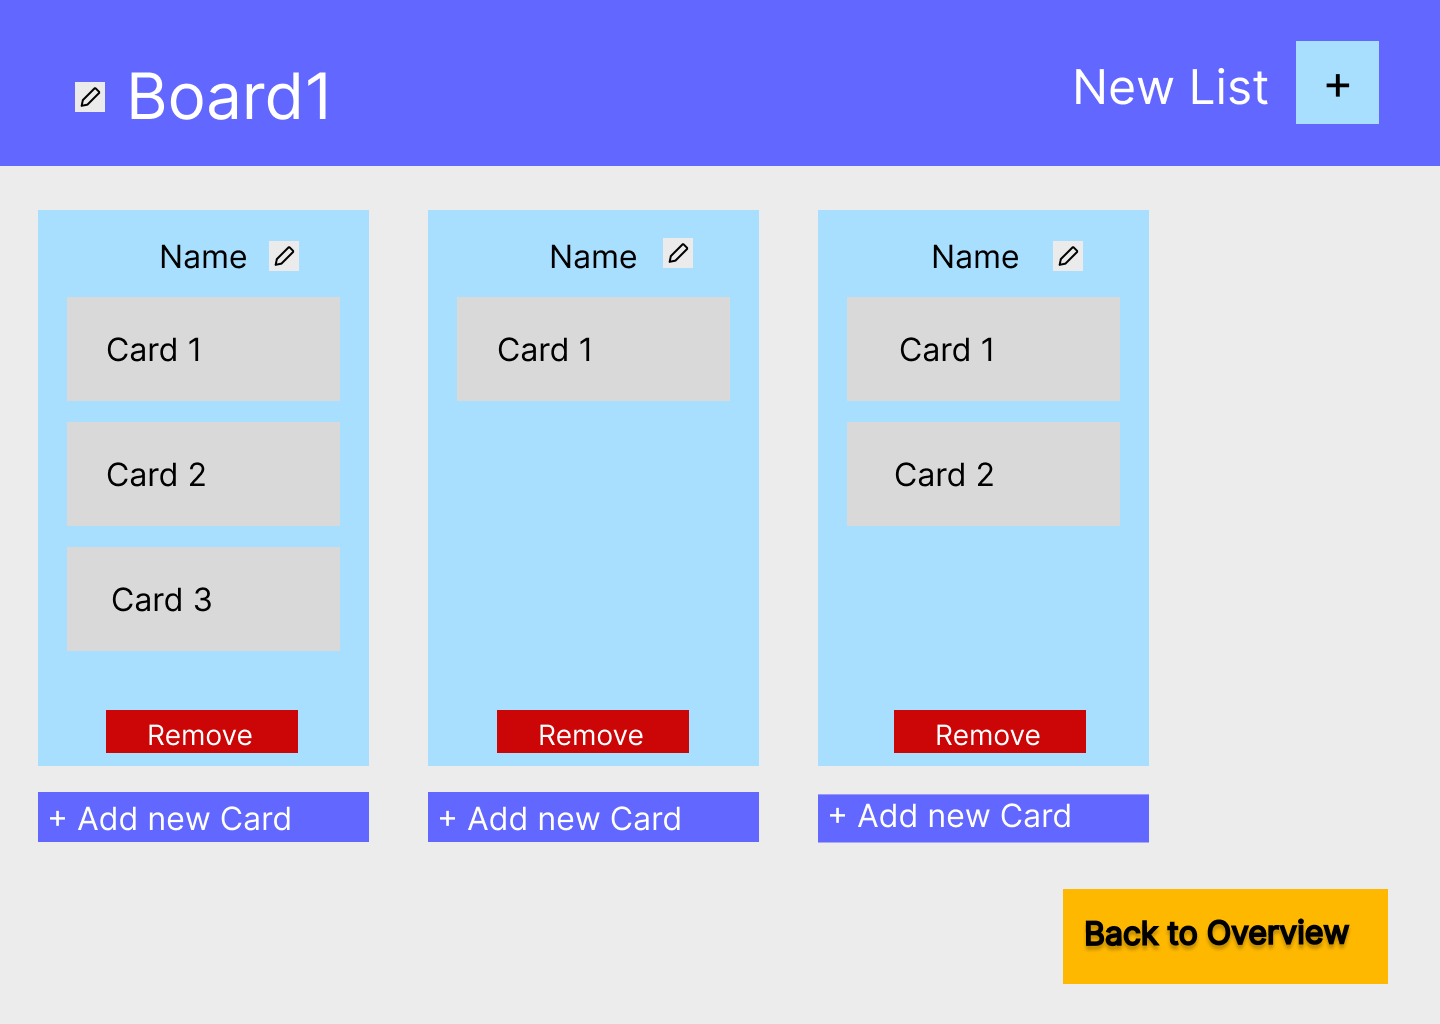
\includegraphics[width=8cm]{content/scenes/Board Overview.png}
\end{figure}

\begin{figure}
    \caption{Card Overview}
    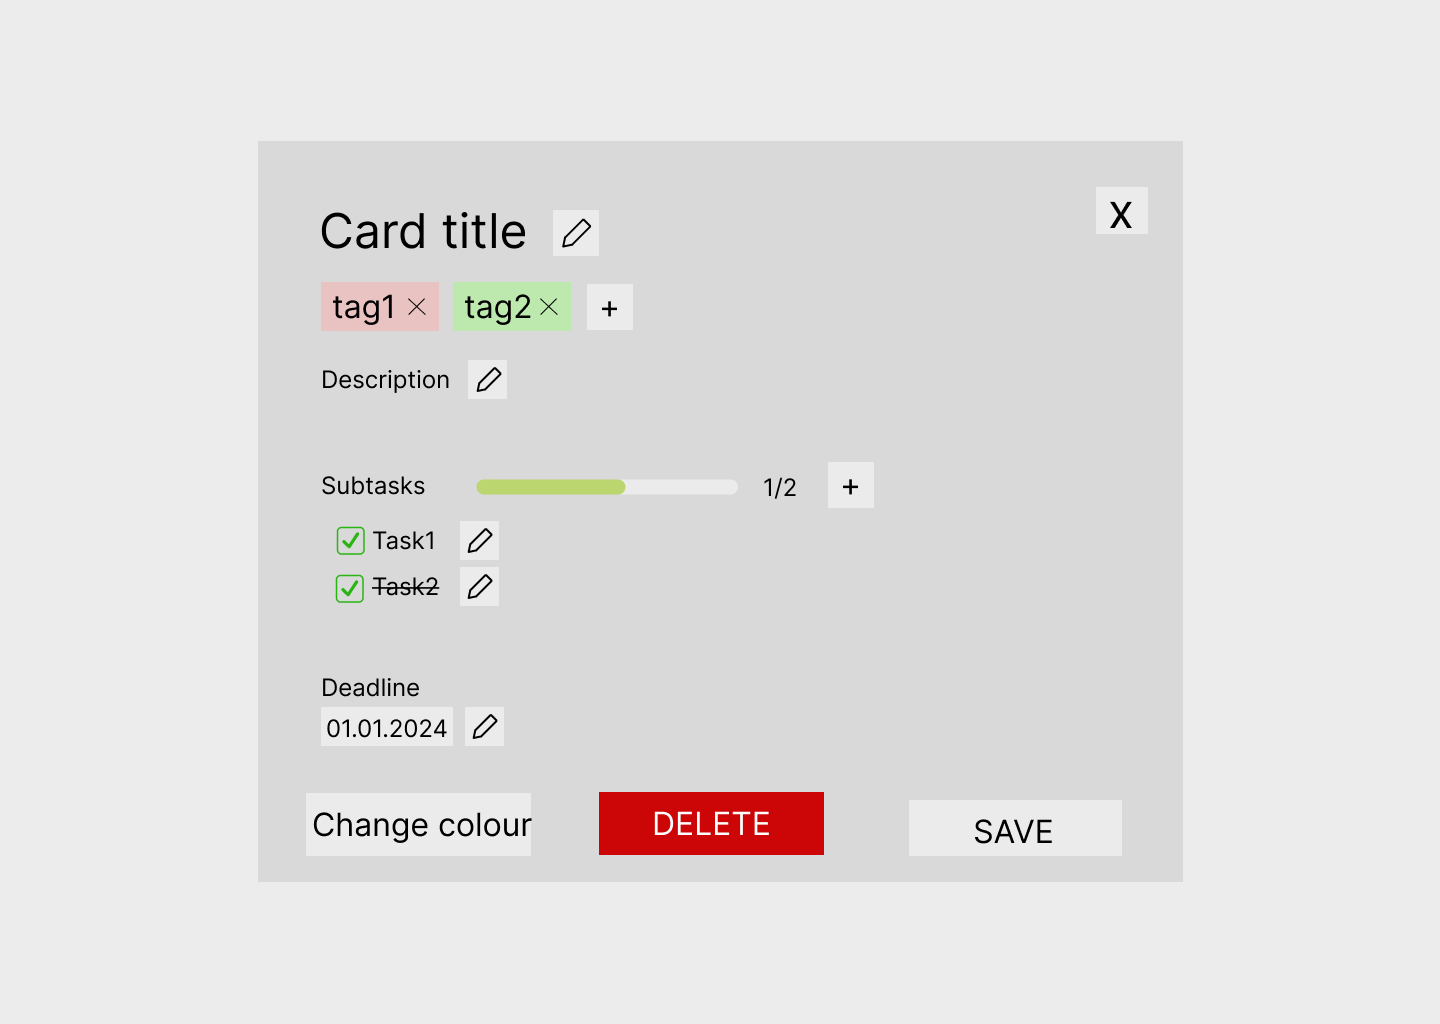
\includegraphics[width=8cm]{content/scenes/Card Overview (Editing).png}
\end{figure}



\begin{figure}
    \caption{Tag Editor}
    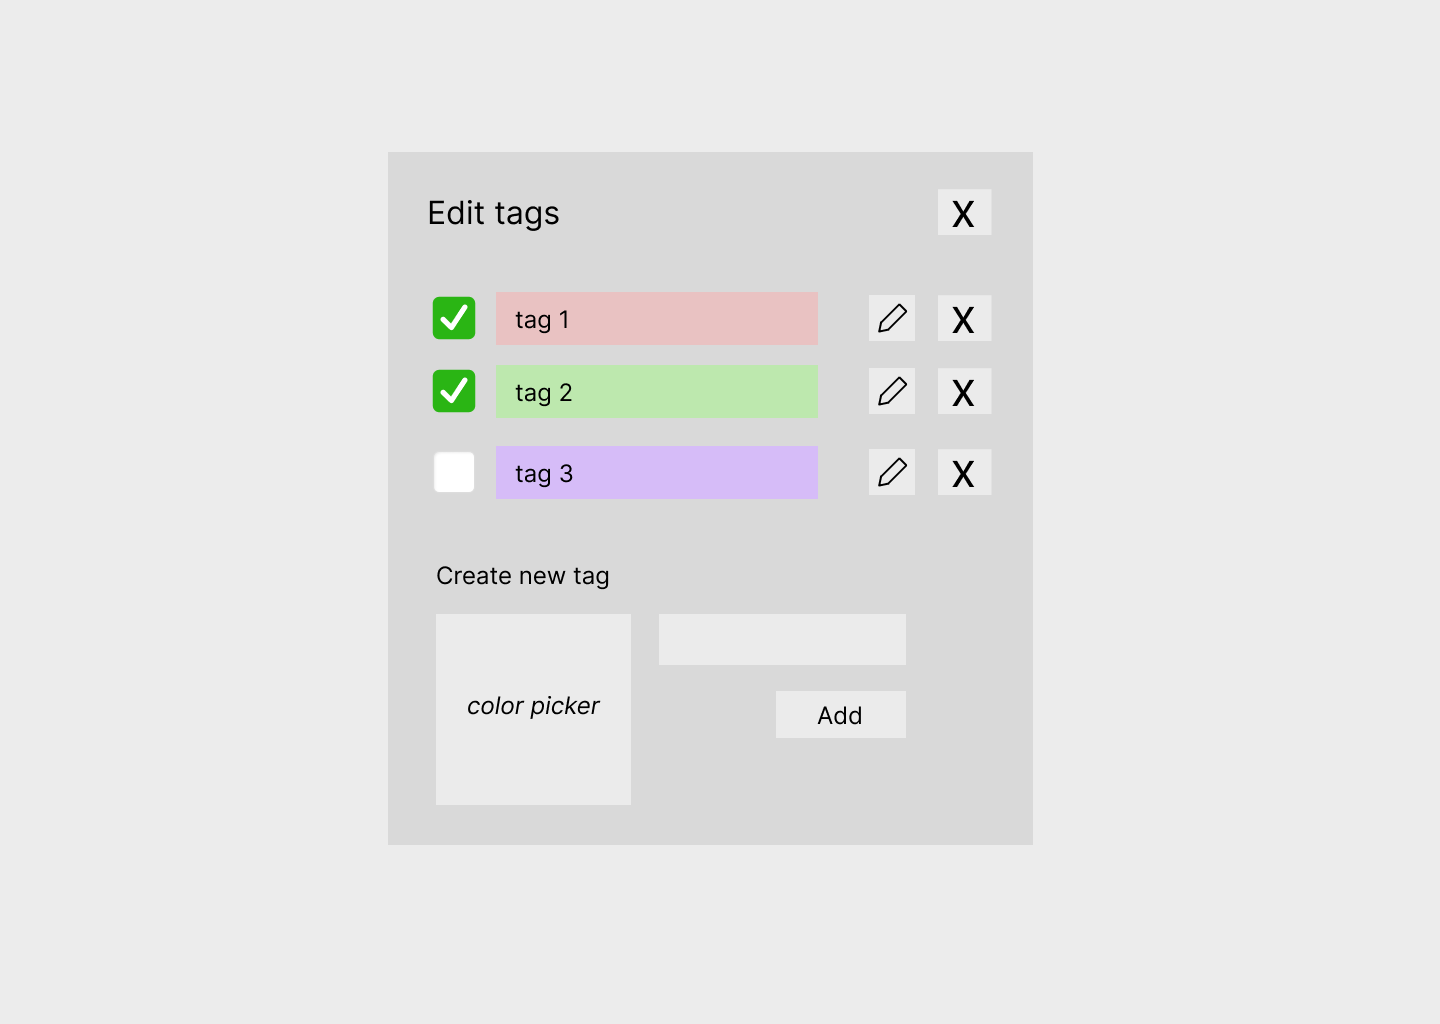
\includegraphics[width=8cm]{content/scenes/Edit tags.png} 
\end{figure}

\begin{figure}
    \caption{Colour Picker}
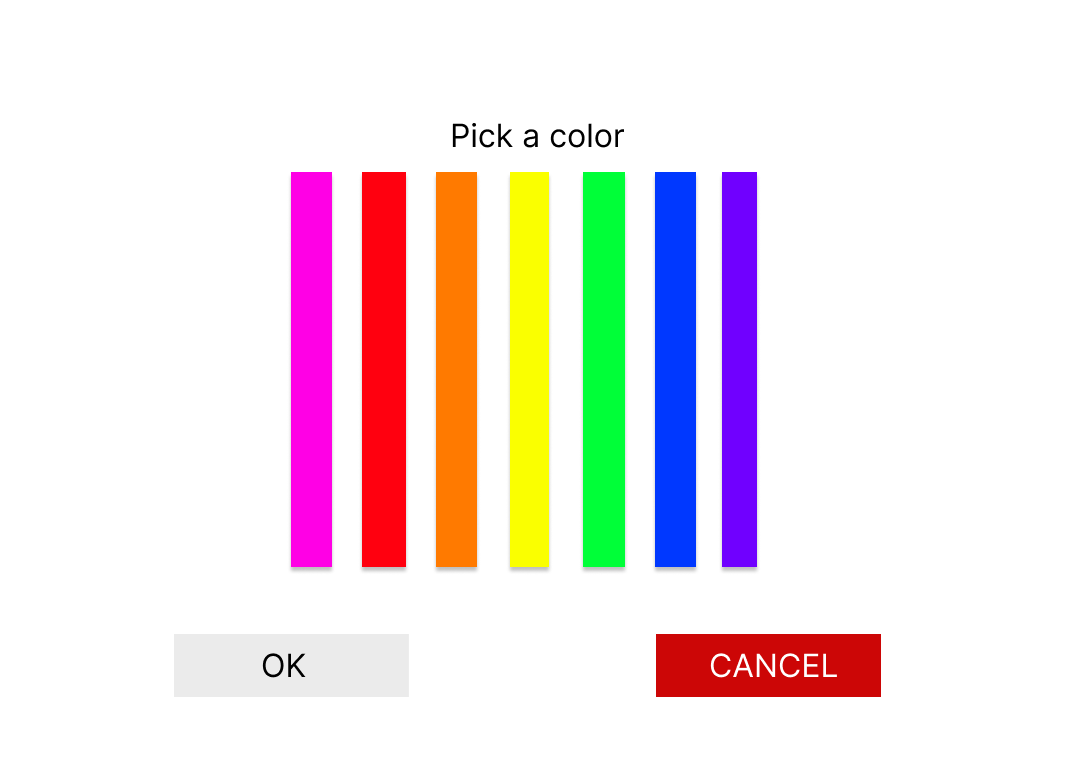
\includegraphics[width=8cm]{content/scenes/Change Colour.png}
\end{figure}

